\documentclass{article}
\pagenumbering{arabic}

\usepackage{url}
\usepackage{color}
\usepackage{verbatim}
\usepackage{tikz}
\usepackage{gnuplot-lua-tikz}

\usepackage{xspace}

%\usepackage[utf8]{inputenc}
%\usepackage{fontspec}
\usepackage{pgfplots}

\usepackage[procnames]{listings}
\lstset{ %
  backgroundcolor=\color{gray98},    % choose the background color; you must add \usepackage{color} or \usepackage{xcolor}
  basicstyle=\tt\small, % \prettysmall      % the size of the fonts that are used for the code
  breakatwhitespace=false,          % sets if automatic breaks should only happen at whitespace
  breaklines=true,                  % sets automatic line breaking
  showlines=true,                  % sets automatic line breaking
  captionpos=b,                     % sets the caption-position to bottom
  commentstyle=\color{gray30},      % comment style
  extendedchars=true,               % lets you use non-ASCII characters; for 8-bits encodings only, does not work with UTF-8
  frame=single,                     % adds a frame around the code
  keepspaces=true,                  % keeps spaces in text, useful for keeping indentation of code (possibly needs columns=flexible)
  keywordstyle=\color{amblu},       % keyword style
  procnamestyle=\color{amred},       % procedures style
  language=[95]fortran,             % the language of the code
  numbers=left,                     % where to put the line-numbers; possible values are (none, left, right)
  numbersep=5pt,                    % how far the line-numbers are from the code
  numberstyle=\tiny\color{gray20}, % the style that is used for the line-numbers
  rulecolor=\color{gray20},          % if not set, the frame-color may be changed on line-breaks within not-black text (e.g. comments (green here))
  showspaces=false,                 % show spaces everywhere adding particular underscores; it overrides 'showstringspaces'
  showstringspaces=false,           % underline spaces within strings only
  showtabs=false,                   % show tabs within strings adding particular underscores
  stepnumber=2,                     % the step between two line-numbers. If it's 1, each line will be numbered
  stringstyle=\color{amblu},       % string literal style
  tabsize=2,                        % sets default tabsize to 2 spaces
  % title=\lstname,                    % show the filename of files included with \lstinputlisting; also try caption instead of title
  procnamekeys={call}
}

\usepackage{color}
\definecolor{gray98}{rgb}{0.98,0.98,0.98}
\definecolor{gray20}{rgb}{0.20,0.20,0.20}
\definecolor{gray25}{rgb}{0.25,0.25,0.25}
\definecolor{gray16}{rgb}{0.161,0.161,0.161}
\definecolor{gray60}{rgb}{0.6,0.6,0.6}
\definecolor{gray30}{rgb}{0.3,0.3,0.3}
\definecolor{bgray}{RGB}{248, 248, 248}
\definecolor{amgreen}{RGB}{77, 175, 74}
% \definecolor{amblu}{RGB}{72, 88, 102}
\definecolor{amblu}{RGB}{55, 126, 184}
\definecolor{amred}{RGB}{228,26,28}
\definecolor{amyellow}{RGB}{237,177,32}
\definecolor{ampurple}{RGB}{126,47,142}
\newcommand{\mye}[1]{\textcolor{amyellow}{#1}\xspace}
\newcommand{\mgr}[1]{\textcolor{amgreen}{#1}\xspace}
\newcommand{\mbl}[1]{\textcolor{amblu}{#1}\xspace}
\newcommand{\mre}[1]{\textcolor{amred}{#1}\xspace}
\newcommand{\mbk}[1]{\textcolor{black}{#1}\xspace}
\newcommand{\mbp}[1]{\textcolor{ampurple}{#1}\xspace}

% This version: August 21st, 2008

%%%%%%%%%%%%%%%%%%%%%%%%%%%%% packages %%%%%%%%%%%%%%%%%%%%%%%%%%%%%%

\usepackage{savesym}
%\usepackage{repdefs,latexsym,longtable,cite}
\usepackage{latexsym,longtable,cite}
\usepackage{accents}
\usepackage{varioref}
\savesymbol{dddot}
\savesymbol{ddddot}
\usepackage{amsmath}
\restoresymbol{TXF}{dddot}
\restoresymbol{TXF}{ddddot}
\usepackage{stfctitlepage}
\usepackage{amssymb}
\usepackage{subfigure}
\usepackage{algorithmic}
\usepackage{algorithm}
\usepackage[usenames,dvipsnames]{pstricks}
\usepackage{epsfig}
\usepackage{pst-grad} % For gradients
\usepackage{pst-plot} % For axes
\usepackage[section]{placeins}
\usepackage{lscape}

%%%%%%%%%%%%%%%%%%%%%%% definitions from repdefs %%%%%%%%%%%%%%%%%%%%%

% formatting

\textwidth  16.17cm 
\textheight 23.4cm
\oddsidemargin -0.2mm 
\evensidemargin -0.2mm
\def\baselinestretch{1.1} 
\topmargin -8.4mm 
\renewcommand{\textfraction}{0.05}
\setlength{\unitlength}{1mm}

% sections

\newcommand{\resetcounters}{\setcounter{equation}{0} \setcounter{figure}{0} 
 \setcounter{table}{0}}
\newcommand{\numsection}[1]{\section{#1}\resetcounters}

% Equations, tables and figures numbered by chapter and section

\renewcommand{\theequation}{\arabic{section}.\arabic{equation}}
\renewcommand{\thetable}{\arabic{section}.\arabic{table}}
\renewcommand{\thefigure}{\arabic{section}.\arabic{figure}}

% displayed equations

\newcommand{\eqn}[2]{\begin{equation}\label{#1}{#2}\end{equation}}
\newcommand{\disp}[1]{\[{#1}\]}
\newcommand{\tim}[1]{\;\; \mbox{#1} \;\;}
\newcommand{\rim}[1]{\;\;\; \mbox{#1} \;\;\;}

% arrays etc

\newcommand{\vect}[1]{\left(\begin{array}{c}#1\end{array}\right)}
\newcommand{\mat}[2]{\left(\begin{array}{#1}#2\end{array}\right)}
\newcommand{\matinv}[2]{\left(\begin{array}{#1}#2\end{array}\right)^{-1}}
\newcommand{\arr}[2]{\begin{array}{#1}#2\end{array}}

% shorthand for itemize, etc

\newcommand{\ite}[1]{\begin{itemize}{#1}\end{itemize}}
\newcommand{\enu}[1]{\begin{enumerate}{#1}\end{enumerate}}
\newcommand{\des}[1]{\begin{description}{#1}\end{description}}

% mathematics

\renewcommand{\Re}{\hbox{I\hskip -1.5pt R}}
\newcommand{\smallRe}
     {\mbox{\raisebox{-0.8pt}{\footnotesize I\hskip -1.5pt R\hskip -0.5pt}}}
\newcommand{\mininx}[1]{ {\renewcommand{\arraystretch}{0.8} 
                     \begin{array}[t]{c} 
                     \mbox{minimize} \vspace*{-1mm} \\ 
                     \mbox{ $\scriptstyle x \in \smallRe^n #1 $ } 
                     \end{array} \;} }
\newcommand{\minin}[1]{ {\renewcommand{\arraystretch}{0.8} 
                     \begin{array}[t]{c} 
                     \mbox{minimize} \vspace*{-1mm} \\ 
                     \mbox{ $\scriptstyle #1 $ } 
                     \end{array} \;} }
\newcommand{\eqdef}{\stackrel{\rm def}{=}}
\newcommand{\bigsum}{\displaystyle \sum}
\newcommand{\bigfrac}[2]{\displaystyle\frac{#1}{#2}}
\newcommand{\s}[1]{^{\mbox{\protect\tiny #1}}}
\newcommand{\sub}[1]{_{\mbox{\protect\tiny #1}}}
\newcommand{\st}{\,\mid\,}
\newcommand{\diag}{\mbox{diag}}

%  fractions

\newcommand{\sfrac}[2]{{\scriptstyle \frac{#1}{#2}}}
\newcommand{\half}{\sfrac{1}{2}}
\newcommand{\quarter}{\sfrac{1}{4}}
\newcommand{\eighth}{\sfrac{1}{8}}

% theorems etc

\newtheorem{theorem}{Theorem}[section]
\newtheorem{lemma}[theorem]{Lemma}
\newtheorem{corollary}[theorem]{Corollary}
\newtheorem{example}{Example}[section]
\newtheorem{defn}{Definition}[section]
\newtheorem{remark}{Remark}[section]
\newtheorem{assumption}{Assumption}[section]
\newcommand{\llem}[2]{\vspace{\baselineskip} 
 \noindent\framebox[\textwidth]{\parbox{0.95\textwidth}{
 \begin{lemma} \label{#1} \rm #2 \end{lemma} } } \vspace{\baselineskip} }
\newcommand{\lthm}[2]{\vspace{\baselineskip} 
 \noindent\framebox[\textwidth]{\parbox{0.95\textwidth}{
 \begin{theorem} \label{#1} \rm #2 \end{theorem} } } \vspace{\baselineskip} }
\newcommand{\lcor}[2]{\vspace{\baselineskip}
 \noindent\framebox[\textwidth]{\parbox{0.95\textwidth}{
 \begin{corollary} \label{#1} \rm #2 \end{corollary} } } \vspace{\baselineskip} }
\newcommand{\lassump}[2]{\vspace{\baselineskip}
 \noindent\framebox[\textwidth]{\parbox{0.95\textwidth}{
 \begin{assumption} \label{#1} \rm #2 \end{assumption} } } \vspace{\baselineskip} }
\newcommand{\ldefn}[2]{\vspace{\baselineskip}
 \noindent\framebox[\textwidth]{\parbox{0.95\textwidth}{
 \begin{defn} \label{#1} \rm #2 \end{defn} } } \vspace{\baselineskip} }

% proofs

\newcommand{\bpr}{{\bf Proof.} \hspace{1.5mm}}
\newcommand{\epr}{\hfill $\Box$ \vspace*{1em}}
\newcommand{\proof}[1]{
\begin{list}{}{
\setlength{\topsep}{0.0pt}
\setlength{\partopsep}{0.0pt}
\setlength{\leftmargin}{0.025\textwidth}
\setlength{\rightmargin}{0.5\leftmargin}
\setlength{\labelwidth}{0.5\leftmargin}
\setlength{\labelsep}{0.25\leftmargin}}
\item \bpr #1 \epr \noindent
\end{list}}

% appendix

\newcommand{\newappendixname}{A}
\newcommand{\newappendix}[1]{\renewcommand{\newappendixname}{{#1}}
 \section*{Appendix \newappendixname} 
 \resetcounters
 \renewcommand{\theequation}{\newappendixname.\arabic{equation}}
 }

% calligraphic letters

\newcommand{\calA}{{\cal A}} \newcommand{\calB}{{\cal B}}
\newcommand{\calC}{{\cal C}} \newcommand{\calD}{{\cal D}}
\newcommand{\calE}{{\cal E}} \newcommand{\calF}{{\cal F}}
\newcommand{\calG}{{\cal G}} \newcommand{\calH}{{\cal H}}
\newcommand{\calI}{{\cal I}} \newcommand{\calJ}{{\cal J}}
\newcommand{\calK}{{\cal K}} \newcommand{\calL}{{\cal L}}
\newcommand{\calM}{{\cal M}} \newcommand{\calN}{{\cal N}}
\newcommand{\calO}{{\cal O}} \newcommand{\calP}{{\cal P}}
\newcommand{\calQ}{{\cal Q}} \newcommand{\calR}{{\cal R}}
\newcommand{\calS}{{\cal S}} \newcommand{\calT}{{\cal T}}
\newcommand{\calU}{{\cal U}} \newcommand{\calV}{{\cal V}}
\newcommand{\calW}{{\cal W}} \newcommand{\calX}{{\cal X}}
\newcommand{\calY}{{\cal Y}} \newcommand{\calZ}{{\cal Z}}

% figures

\newcommand{\fig}[2]{\begin{figure}[htbp]
\begin{center} {#1} \caption{#2} \end{center} \end{figure}}
\newcommand{\figt}[2]{\begin{figure}[t]
\begin{center} {#1} \caption{#2} \end{center} \end{figure}}


%%%%%%%%%%%%%%%%%%%%%%% additional definitions %%%%%%%%%%%%%%%%%%%%%%%

\newcommand{\mycitetwo}[4]{[\citenum{#1}: #2, \citenum{#3}: #4]}
\newcommand{\mycitethree}[3]{[\citenum{#1}: #2, \citenum{#3}]}

\newcommand{\lk}{\lambda_k}
\newcommand{\lkp}{\lambda_{k+1}}
\newcommand{\dk}{\delta_k}

\newcommand{\lambdac}{\lambda\sub{C}}
\newcommand{\lambdae}{\lambda\sub{E}}
\newcommand{\lambdas}{\lambda\sub{S}}
\newcommand{\lambdal}{\lambda\sub{L}}
\newcommand{\lambdat}{\lambda\sub{T}}
\newcommand{\lambdau}{\lambda\sub{U}}
\newcommand{\xs}{x\sub{S}}
\newcommand{\alphas}{\alpha\sub{S}}
\newcommand{\thetal}{\theta\sub{L}}
\newcommand{\thetau}{\theta\sub{U}}

\newcommand{\xl}{x(\lambda)}
\newcommand{\xlt}{x^T(\lambda)}
\newcommand{\xlp}{\dot{x}(\lambda)}
\newcommand{\xlpt}{\dot{x}^T(\lambda)}
\newcommand{\xlpp}{\ddot{x}(\lambda)}
\newcommand{\xlppt}{\ddot{x}^T(\lambda)}

\newcommand{\xlz}{x^{(0)}(\lambda)}
\newcommand{\xlo}{x^{(1)}(\lambda)}
\newcommand{\xlk}{x^{(k)}(\lambda)}
\newcommand{\xlkt}{x^{(k)T}(\lambda)}
\newcommand{\xlkm}{x^{(k-1)}(\lambda)}
\newcommand{\xlkp}{x^{(k+1)}(\lambda)}
\newcommand{\xlkpt}{x^{(k+1)T}(\lambda)}
\newcommand{\xlkpp}{x^{(k+2)}(\lambda)}

\newcommand{\ylz}{y^{(0)}(\lambda)}
\newcommand{\ylk}{y^{(k)}(\lambda)}
\newcommand{\ylkt}{y^{(k)T}(\lambda)}
\newcommand{\ylkp}{y^{(k+1)}(\lambda)}
\newcommand{\ylkpt}{y^{(k+1)T}(\lambda)}
\newcommand{\ylkm}{y^{(k-1)}(\lambda)}

\newcommand{\zlz}{z^{(0)}(\lambda)}
\newcommand{\zlk}{z^{(k)}(\lambda)}
\newcommand{\zlkp}{z^{(k+1)}(\lambda)}
\newcommand{\zlkm}{z^{(k-1)}(\lambda)}

\newcommand{\Hlm}{H + \lambda M}
\newcommand{\Hlmc}{H + \lambdac M}

\newcommand{\pil}{\pi(\lambda)}
\newcommand{\pilp}{\pi^{(1)}(\lambda)}
\newcommand{\pilpp}{\pi^{(2)}(\lambda)}
\newcommand{\pilppp}{\pi^{(3)}(\lambda)}
\newcommand{\pilpppp}{\pi^{(4)}(\lambda)}

%\newcommand{\pilp}{\dot{\pi}(\lambda)}
%\newcommand{\pilpp}{\ddot{\pi}(\lambda)}
%\newcommand{\pilppp}{\dddot{\pi}(\lambda)}
%\newcommand{\pilpppp}{\ddddot{\pi}(\lambda)}

\newcommand{\pitkp}{\pi^{(2k+1)}(\lambda)}
\newcommand{\pitkpt}{\pi^{(2k+2)}(\lambda)}

\newcommand{\yl}{y(\lambda)}
\newcommand{\ylp}{\dot{y}(\lambda)}
\newcommand{\ylpt}{\dot{y}^T(\lambda)}
\newcommand{\ylpp}{\ddot{y}(\lambda)}
\newcommand{\ylppt}{\ddot{y}^T(\lambda)}

\newcommand{\zl}{z(\lambda)}
\newcommand{\zlp}{\dot{z}(\lambda)}
\newcommand{\zlpt}{\dot{z}^T(\lambda)}
\newcommand{\zlpp}{\ddot{z}(\lambda)}
\newcommand{\zlppt}{\ddot{z}^T(\lambda)}

%\newcommand{\baru}{\bar{u}}
%\newcommand{\barx}{\bar{x}}
%\newcommand{\barz}{\bar{z}}
%\newcommand{\barc}{\bar{c}}
%\newcommand{\barH}{\bar{H}}
\newcommand{\barc}{\skew4\overline c}
\newcommand{\barr}{\skew1\overline r}
\newcommand{\baru}{\skew0\overline u}
\newcommand{\barw}{\skew0\overline w}
\newcommand{\barx}{\skew1\overline x}
\newcommand{\bary}{\skew1\overline y}
\newcommand{\barz}{\skew2\overline z}
\newcommand{\barH}{\skew4\overline H}
\newcommand{\barU}{\skew1\overline U}
\newcommand{\hatH}{H\sub{S}}
\newcommand{\hatM}{M\sub{S}}
\newcommand{\hatu}{u\sub{S}}
\newcommand{\hatlambdal}{\lambda\sub{SL}}
%\newcommand{\Dlambda}{\Delta \lambda}
\newcommand{\Dlambda}{\delta}
\newcommand{\Dlambdac}{\delta\sub{C}}

 \newcommand{\mnorm}[1]{\|#1\|_M}

\newcommand{\bovt}{\sfrac{\beta}{2}}

% replace the next two by the best lower bounds for quadratic and cubic approx

\newcommand{\bestq}{-\sfrac{2}{3}}
\newcommand{\bestc}{-\sfrac{2}{5}}
\newcommand{\Real}{\mathbb{R}}

\newcommand{\ud}{\mathrm{d}}
\newcommand{\uu}{\mathbf{u}}
\newcommand{\ff}{\mathbf{f}}
\newcommand{\bb}{\mathbf{b}}
\newcommand{\dd}{\mathbf{d}}

%%%%%%%%%%%%%%%%%%%%%%%% Added by Sue %%%%%%%%%%%%%%%%%%%%%%%%%%%%%%%

\newcommand{\etl}{\eta(\lambda;\beta)}
\newcommand{\etlp}{\eta^{(1)}(\lambda;\beta)}
\newcommand{\etlpp}{\eta^{(2)}(\lambda;\beta)}
\newcommand{\etlppp}{\eta^{(3)}(\lambda;\beta)}
\newcommand{\etlpppp}{\eta^{(4)}(\lambda;\beta)}


\newcommand{\zetl}{\zeta(\lambda;\beta)}
\newcommand{\zetlp}{\zeta^{(1)}(\lambda)}
\newcommand{\zetlpp}{\zeta^{(2)}(\lambda)}
\newcommand{\zetlppp}{\zeta^{(3)}(\lambda)}
\newcommand{\zetlpppp}{\zeta^{(4)}(\lambda)}

%\newcommand{\etlp}{\dot{\eta}(\lambda)}
%\newcommand{\etlpp}{\ddot{\eta}(\lambda)}
%\newcommand{\etlppp}{\dddot{\eta}(\lambda)}
%\newcommand{\etlpppp}{\ddddot{\eta}(\lambda)}

\newcommand{\rhl}{\rho(\lambda)}
\newcommand{\rhlp}{\rho^{(1)}(\lambda)}
\newcommand{\rhlpp}{\rho^{(2)}(\lambda)}
\newcommand{\rhlppp}{\rho^{(3)}(\lambda)}
\newcommand{\rhlpppp}{\rho^{(4)}(\lambda)}

%\newcommand{\rhlp}{\dot{\rho}(\lambda)}
%\newcommand{\rhlpp}{\ddot{\rho}(\lambda)}
%\newcommand{\rhlppp}{\dddot{\rho}(\lambda)}
%\newcommand{\rhlpppp}{\ddddot{\rho}(\lambda)}

\newcommand{\pilb}{\pi(\lambda; \beta)}
\newcommand{\pilbp}{\pi^{(1)}(\lambda; \beta)}
\newcommand{\pilbpp}{\pi^{(2)}(\lambda; \beta)}
\newcommand{\pilbppp}{\pi^{(3)}(\lambda; \beta)}
\newcommand{\pilbpppp}{\pi^{(4)}(\lambda; \beta)}

%\newcommand{\psilp}{\dot{\psi}(\lambda; \beta)}
%\newcommand{\psilpp}{\ddot{\psi}(\lambda; \beta)}
%\newcommand{\psilppp}{\dddot{\psi}(\lambda; \beta)}
%\newcommand{\psilpppp}{\ddddot{\psi}(\lambda; \beta)}

\newcommand{\lam}{\lambda}
\newcommand{\lammax}{\lambda_{\max}}
\newcommand{\lammin}{\lambda_{\min}}
\newcommand{\lami}{\lambda_i}
\newcommand{\lamj}{\lambda_j}
\newcommand{\lamk}{\lambda_k}
\newcommand{\laml}{\lambda_l}
\newcommand{\lamlami}[1]{\left(\lambda + \lambda_i\right)^{#1}}
\newcommand{\lamlamj}[1]{\left(\lambda + \lambda_j\right)^{#1}}
\newcommand{\lamlamk}[1]{\left(\lambda + \lambda_k\right)^{#1}}
\newcommand{\lamlaml}[1]{\left(\lambda + \lambda_l\right)^{#1}}
\newcommand{\sigmax}{\sigma_{\max}}
\newcommand{\sigmin}{\sigma_{\min}}
\newcommand{\mumax}{\mu_{\max}}
\newcommand{\mumin}{\mu_{\min}}

%%%%%%%%%%%%%%%%%%%%%%% Added by Daniel %%%%%%%%%%%%%%%%%%%%%%%%%%%%%%

 %\usepackage{amssymb}

 \newcommand{\sgap}{\;}
 \newcommand{\mgap}{\;\;}
 \newcommand{\bgap}{\;\;\;}
 \newcommand{\cbar}{\skew5\bar c}
 \newcommand{\gammabar}{\bar\gamma}
 \newcommand{\lamA}{\lambda^{\scriptscriptstyle A}}
 \newcommand{\lamR}{\lambda^{\scriptscriptstyle R}}
 \newcommand{\lamone}{\lambda_1}
 \newcommand{\lamtwo}{\lambda_2}
 \newcommand{\lamnext}{\lambda_J}
 \newcommand{\uone}{u_1}
 \newcommand{\nInv}{n}
 \newcommand{\nInvbar}{\bar \nInv}
 \newcommand{\gap}[1]{\text{gap($#1$)}}
 \newcommand{\plusminus}{{\scriptscriptstyle (-/+)\thinspace}}
 \newcommand{\eps}{\varepsilon}
 \newcommand{\northog}{\mathchar"3236 \hspace{-3.5pt} \bot}
\newcommand{\norm}[1]{\left\Vert#1\right\Vert}
\newcommand{\snorm}[1]{\Vert#1\Vert}
\newcommand{\abs}[1]{\left\vert#1\right\vert}
 %\newcommand{\eig}{\mathop{\operator@font{eig}}}
 \newcommand{\eig}{\mathop{\mathrm{eig}}}
 \newcommand{\qbar}{\bar q}
 \newcommand{\lwords}[1]{\text{#1}\mgap}     % text automatically adjusts the size
 \newcommand{\rwords}[1]{\mgap\text{#1}}
 \newcommand{\lwordss}[1]{\text{#1}\quad}    % text automatically adjusts the size
 \newcommand{\rwordss}[1]{\quad\text{#1}}
 \newcommand{\lwordsss}[1]{\text{#1}\qquad}  % text automatically adjusts the size
 \newcommand{\rwordsss}[1]{\qquad\text{#1}}
 \newcommand{\words}[1]{\mgap\text{#1}\mgap}
 \newcommand{\wordss}[1]{\quad\text{#1}\quad}
 \newcommand{\wordsss}[1]{\qquad\text{#1}\qquad}
 
 \newcommand{\alg}[1]{\par\noindent\mystrut\ignorespaces\hbox to\textwidth{#1\hfill}}
 \newcommand{\algt}[1]{\par\noindent\mystrut\hbox to\textwidth{\ignorespaces\hskip1.5em#1\hfill}}
 \newcommand{\algtt}[1]{\par\noindent\mystrut\hbox to\textwidth{\ignorespaces\hskip3.5em#1\hfill}}
 \newcommand{\algttt}[1]{\par\noindent\mystrut\hbox to\textwidth{\ignorespaces\hskip5.5em#1\hfill}}
 \newcommand{\algtttt}[1]{\par\noindent\mystrut\hbox to\textwidth{\ignorespaces\hskip7.5em#1\hfill}}
 \newcommand{\algttttt}[1]{\par\noindent\mystrut\hbox to\textwidth{\ignorespaces\hskip9.5em#1\hfill}}
 \newcommand{\clg}[2]{\par\noindent\mystrut\hbox to\textwidth{\ignorespaces#1\hfill[#2]}}
 \newcommand{\clgt}[2]{\par\noindent\mystrut\hbox to\textwidth{\ignorespaces\hskip1.5em#1\hfill[#2]}}
 \newcommand{\clgtt}[2]{\par\noindent\mystrut\hbox to\textwidth{\ignorespaces\hskip3.5em#1\hfill[#2]}}
 \newcommand{\clgttt}[2]{\par\noindent\mystrut\hbox to\textwidth{\ignorespaces\hskip5.5em#1\hfill[#2]}}
 \newcommand{\clgtttt}[2]{\par\noindent\mystrut\hbox to\textwidth{\ignorespaces\hskip7.5em#1\hfill[#2]}}
 \newcommand{\clgttttt}[2]{\par\noindent\mystrut\hbox to\textwidth{\ignorespaces\hskip9.5em#1\hfill[#2]}}
 \newcommand{\mystrut}{\vrule height9.5pt depth1.5pt width0pt}
 \newtheorem{definition}{Definition}[section]

 \newcounter{pseudocode}[section]
 \def\thepseudocode{\thesection.\arabic{pseudocode}}
 \newenvironment{pseudocode}[2]%
	{%
	\refstepcounter{pseudocode}%
	\vspace{\medskipamount}\noindent 
               {{\sc       Algorithm \thepseudocode.} \rule[-1.25pt]{0pt}{10pt}\sc#1}%
%              {{\bfseries Algorithm \thepseudocode.} \rule[-1.25pt]{0pt}{10pt}\slshape#1}%
%              {{\bfseries Algorithm \thepseudocode.} \rule[-1.25ex]{0pt}{2ex}\slshape#1}%
	#2}%
	{\vspace{\medskipamount}}

\ifx   \innerprod\undefined%
   \def\innerprod(#1,#2){\langle#1,#2\rangle} % Must be called as \innerproduct(A,B)
\fi


\newcommand{\alert}[1]{\textcolor{red}{#1}\xspace}
\newcommand{\starpu}{{StarPU}\xspace}
\newcommand{\parsec}{{PaRSEC}\xspace}
\newcommand{\TODO}{\alert{TODO}\xspace}
\newcommand{\openmp}{OpenMP\xspace}
\newcommand{\ma}{HSL\_MA87\xspace}
\newcommand{\spllt}{SpLLT\xspace}

\bibliographystyle{siam}

%-----------------------------------------------------------------------
%
% include macros
%
\input nlafet_macros.tex
%-----------------------------------------------------------------------



\newcommand{\stfccovertitle}
{Experiments with sparse Cholesky using runtime systems}


\newcommand{\theabstract}{We describe the development of a prototype code for 
the solution of large symmetric positive definite sparse systems that is
efficient on parallel architectures.
}

\textwidth  16.18cm
\textheight 23.4cm
\oddsidemargin -0.2mm
\evensidemargin -0.2mm
\def\baselinestretch{1.1}
\topmargin -8.4mm

\newcommand{\n}[1][1]{\vspace*{#1\baselineskip}\noindent}
\newcommand{\ISD}[1]{\begin{center}\n[.4]\textcolor{red}{ISD\
 \hspace*{0.15em} \fbox{\parbox{.8\textwidth}{#1}}}\n[.4]\end{center}}
\newcommand{\HSD}[1]{\begin{center}\n[.4]\textcolor{green}{FL\
\hspace*{0.15em} \fbox{\parbox{.9\textwidth}{\texttt{#1}}}}\n[.4]\end{center}}
\newcommand{\ASH}[1]{\begin{center}\n[.4]\textcolor{brown}{JH\
\hspace*{0.15em} \fbox{\parbox{.9\textwidth}{\texttt{#1}}}}\n[.4]\end{center}}

\newcommand{\metis}{{\sc Me$\!$T$\!$iS\ }}

\hyphenpenalty=10000
\widowpenalty=10000
\sloppy

\begin{document}


\begin{titlepage}

\vspace*{-0.5cm}

\vspace{1.0 cm}

{\Large \bf
\begin{center}
   \stfccovertitle
\end{center}}

\begin{center}
\mbox{} \\
      Iain Duff, 
      Jonathan Hogg, and Florent Lopez
     
\mbox{} \\
\end{center}

\vspace{1.0cm}


\noindent
{\large ABSTRACT}

\vspace{0.3cm}
\noindent
\theabstract

\vspace{0.6cm}

\begin{description}
\item [Keywords:] sparse Cholesky, SPD systems, runtime systems, STARPU, OpenMP
\item [AMS(MOS) subject classifications:]  65F30, 65F50
\end{description}

\vspace{0.1 cm}

\noindent \rule{15cm}{0.001in}
\vspace{0.1 cm}

\begin{description}

\item Scientific Computing Department, STFC Rutherford Appleton
  Laboratory, Harwell Campus,\\ Oxfordshire, OX11 0QX, UK.
\end{description}
\noindent
Correspondence to: florent.lopez@stfc.ac.uk\\
This work was supported by the FET-HPC H2020 NLAFET grant number xxxx.\\


\vspace{1.1 cm}
\noindent \today

\end{titlepage}

\newpage
\setcounter{page}{1}
\pagenumbering{arabic}

\section{Introduction} \label{sec:introduction} 



We investigate the use of a runtime system for the implementation of a
sparse Cholesky solver used to find the solution of the linear system:
\begin{equation}\label{eq:linear-system}
  Ax = b
\end{equation}
where $A$ is a large sparse symmetric positive-definite matrix. We
particularly focus on exploiting multicore architectures that have
become increasingly popular since their introduction and can be found
nowadays in the vast majority of high performance computing
platforms. Despite their popularity, exploiting the capabilities of
multicore processors remains a challenge and to cope with multicore
hardware, DAG-based algorithms have been shown to be extremely
efficient in terms of performance and scalability. Initially they have
been employed in the context of dense linear algebra such as in the
PLASMA software package~\cite{a.d.d.h.ea:09}, motivated by the high
efficiency provided by these algorithms. They have been adapted to
sparse algorithms in for example of the \texttt{HSL\_MA87}
solver~\cite{h.r.s:10} that implements a DAG-based sparse supernodal
Cholesky factorization and the \texttt{qr\_mumps} solver~\cite{b:13}
that implements a DAG-based multifrontal QR method.

The traditional approach for implementing a task-based solver includes
the development of an ad hoc scheduler which relies on the knowledge
of the algorithm and is implemented using a low-level multithreading
library such as pthread (POSIX threads) to manage synchronisations and
enforce dependencies between processes. This approach however causes a
lack of portability of the implemented software as it is developed for
a given target architecture, it can then be costly in terms of
programming effort to port the code to different architectures and
adapt to the emerging ones. This problem occurs, for example, when
targeting heterogeneous architectures such as GPU-accelerated
multicore systems that have a more complex memory hierarchy than
traditional multicore systems and equipped different types of
processing units with different capabilities. Instead, in this work,
we explore an alternative approach based on the use of a runtime
system which consists of a software layer between the architecture and
the application. In this context the application is implemented using
a high-level API provided by the runtime system and low level details
such as data consistency across the architecture and task scheduling
are delegated to the runtime system. We focus on the exploitation of a
Sequential Task Flow (STF) programming model for expressing the DAG
corresponding to our application. We show that our code, implemented
with a task-based runtime system, can lead to an implementation of a
sparse matrix factorization which is as efficient as a
state-of-the-art solver on a multicore system.

\section{Task-based sparse Cholesky factorization}\label{sec:chol}
\setcounter{equation}{0}
\setcounter{table}{0}
\setcounter{figure}{0}

We first describe the supernodal Cholesky factorization method that we
use for solving sparse symmetric positive-definite systems. In
particular we will focus on a DAG-based variant of this algorithm that
has been proven to be extremely efficient on multicore architectures
such as for example the \ma solver~\cite{h.r.s:10}.

The supernodal Cholesky method is a factorization algorithm for sparse
matrices where the input matrix $A$ is decomposed as:
\begin{equation}\label{eq:chol}
  A = LL^{T}
\end{equation}
where the factor $L$ is a lower triangular matrix. Note that the
sparsity pattern of the factor is not the same as the original matrix
as because additional coefficients generally appear during the
computation of this factor resulting in a denser matrix than the
original one. This phenomenon is called \textit{fill-in} and can be
greatly reduced by the use of a symmetric permutation applied to the
matrix before the factorization. If, for example, we apply the
symmetric permutation $P$ to the matrix $A$ then we transform the
original matrix into $PAP^{T}$. The dependencies between the
coefficients in the factor $L$ during the factorization can be
expressed in a tree structure called an \textit{elimination tree}
where each node in this tree represent a column in the factor. In
order to increase the efficiency of operations by exploiting Level 3
BLAS routines, the elimination tree is transformed into an
\textit{assembly tree} where columns having a similar nonzero pattern
are amalgamated into a dense matrix that is referred to a
\textit{nodal} matrix or \textit{supernode}. The factorization is
effected by traversing the assembly tree in a topological order and
performing two main operations at each supernode: a dense Cholesky
factorization of the current supernode and an update of the ancestor
supernodes using the computed factors in the nodal factorization. The
update operations may be performed according to several strategies:
\textit{right-looking} updates where ancestors nodes are updated as
soon as the nodal factorization is done, or \textit{left-looking}
updates where the current supernode is updated just before being
factorized. The assembly tree is computed during an analysis phase
preceding the factorization and in our case we obtain it by using the
software package HSL\_MC78 \alert{find reference for MC78}.

There are two main sources of parallelism that can be exploited in the
assembly tree which are the \textit{tree-level} and
\textit{node-level}. The tree-level parallelism is due to the fact
that supernodes located in separate branches of the tree can be
processed independently and the node-level parallelism is exploited
when nodes are large enough and can be processed by multiple resources
in parallel. One approach for the parallelization of the supernodal
algorithm consists in exploiting these two levels of parallelism
separately \alert{give more explanation about this
  strategy. Separately is misleading} . Instead, in our work, we
follows the approach proposed in~\cite{h.r.s:10} where supernodes are
partitioned into square blocks of order \texttt{nb} and operations are
applied on these blocks. Figure~\ref{fig:etree-simple-part} shows a
simple assembly tree that consists of three supernodes where the
dashed lines represent the block partitioning of
supernodes. Figures~\ref{fig:dag-simple} represent the DAG associated
with the factorization of the tree presented in
Figure~\ref{fig:etree-simple-part}.

\begin{figure}[!h]
  \begin{minipage}{0.5\textwidth}
    \centering
    \includegraphics[width=0.7\textwidth]{figures/etree_simple_part}
    \caption{\label{fig:etree-simple-part}Simple assembly tree with
      three supernodes partitioned into square blocks of order
      \texttt{nb}.}
  \end{minipage}
  \hspace{0.5cm}
  \begin{minipage}{0.5\textwidth}
    \centering
    \includegraphics[width=0.7\textwidth]{figures/dag}
    \caption{\label{fig:dag-simple} DAG corresponding to the
      factorization of the tree in Figure~\ref{fig:etree-simple-part}.}
  \end{minipage}
\end{figure}

As shown in the DAG represented in Figure~\ref{fig:dag-simple} they
are several kernels involved in the factorization of the supernodes:
the tasks denoted \texttt{f} correspond to the computation of the
Cholesky factor of a diagonal block. Tasks denoted \texttt{s} perform
a triangular solve of a subdiagonal block using a factor computed with
a task \texttt{f}. Tasks denoted \texttt{u} perform an update of a
block within a supernode with respect to the previous factorization of
blocks. Finally, tasks denoted \texttt{a} represent the update between
supernodes with respect to the factorization blocks computed in a
given node. 
  % For more details on the kernels, we refer
% to~\cite{h.r.s:10}.

In our code, the DAG, such as the one presented in
Figure~\ref{fig:dag-simple}, replaces the elimination tree for
expressing the dependencies during the computation of factors. Note
that when exploiting separately the node and tree parallelism, it is
not possible to start factorizing a supernode before all of its
descendant have been processed. However, when using the DAG, it is
possible that some tasks in a given node become ready for execution
and are then scheduled while its descendent are still being
processed. Using this DAG-based parallelism it is therefore possible
to pipeline the processing of a given node with the processing of it
ancestors. This additional level of parallelism allowed by the use of
a DAG-based algorithm is referred to as inter-node parallelism.
 
\section{Sequential Task Flow parallel programming model}\label{sec:stf-model}

In this work we propose exploiting a \textit{Sequential Task Flow
  (STF)} programming model for the implementation of a parallel
task-based Cholesky factorization on top of a runtime system. In this
model the detection of dependencies between tasks relies on a data
analysis of input and output data in order to guarantee the
\textit{sequential consistency} of operations during a parallel
execution. This analysis is often referred to as a
\textit{superscalar} analysis in reference to the dependency detection
between instructions that are performed in superscalar processors. In
this context the dependency graph is used to allow the parallel
execution of independent instructions which is referred to as
instruction-level parallelism and increases the instruction
throughput. The STF model is the most commonly used paradigm for the
parallelization of DAG-based algorithms that have become more and more
popular in the scientific computing community. For example, several
dense linear algebra software packages such as
PLASMA~\cite{a.d.d.h.ea:09} and FLAME~\cite{i.c.q.q.ea:12} use this
paradigm in their implementation. One reason for such a popularity is
that it is extremely easy to use this model as the parallel code is
very similar to the sequential one. Essentially, for a given
sequential algorithm, the STF code is implemented by replacing the
function calls (i.e. the execution of tasks in the case of a DAG-based
algorithm) with the asynchronous submission of this task to a runtime
system in charge of the scheduling. Depending on the data access
provided, the runtime system automatically detects the dependencies
between the tasks. The sequential consistency is then ensured by the
fact that the order of submission of tasks corresponds to the
sequential order.

\begin{figure}[!h]
  \begin{minipage}{0.5\textwidth}
    \centering \lstset{language=C, procnamekeys={}}
    \lstinputlisting{listings/seq-example.c}
    \caption{\label{fig:seq-example}Simple of a sequential code}
    \vspace{0.5cm}
    \centering \lstinputlisting{listings/stf-example.c}
    \caption{\label{fig:stf-example}STF code}
  \end{minipage}
  \hspace{0.5cm}
  \begin{minipage}{0.5\textwidth}
    \centering
    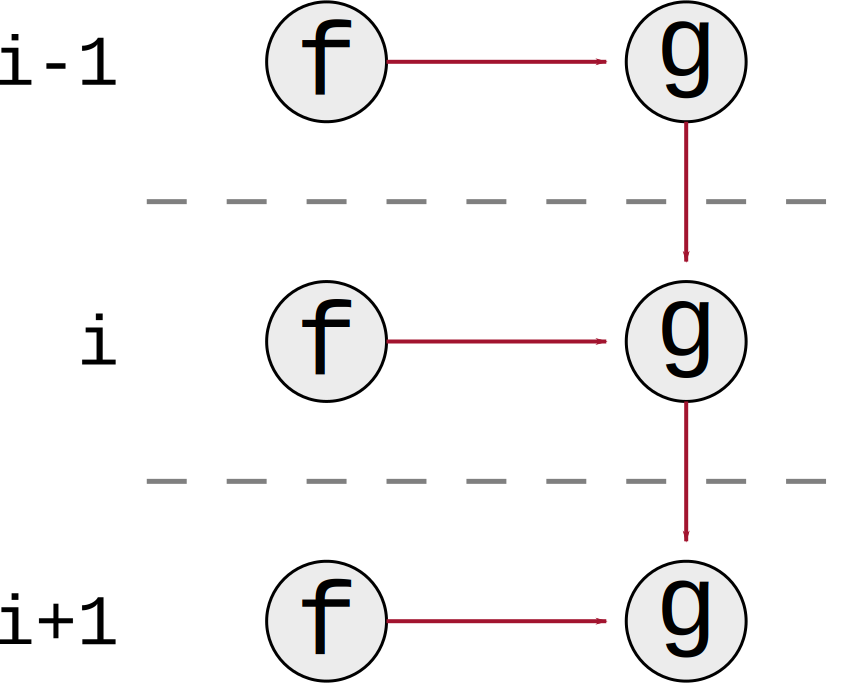
\includegraphics[width=0.7\textwidth]{figures/example_dag}
    \caption{\label{fig:dag-example}DAG corresponding to the
      sequential code presented in Figure~\ref{fig:stf-example}}
  \end{minipage}
  %% \caption{\label{fig:seq-example} Simple example of a sequential code
  %%   on the left with the corresponding DAG represented on the right.}
\end{figure}

As an example, we consider the sequential code in
Figure~\ref{fig:seq-example} for which the corresponding DAG is
represented in Figure~\ref{fig:dag-example}. Based on a STF model, the
parallel version of this code is illustrated in
Figure~\ref{fig:stf-example}. In the sequential code, the two
functions \textit{f} and \textit{g} manipulate arrays \textit{x} and
\textit{y}. The STF code is obtain by submitting the tasks that
consist of a kernels funtion (\textit{f} or \textit{g} in this
example) together with data which are associated with a data access
which can be \textit{R} when the data is read, \textit{W} when the
data is modified, and \textit{RW} when the data is read and modified.

As we have seen with this simple example, the STF model is extremely
easy to use and this characteristic is certainly one of the main
reasons for its popularity in the HPC community. This model, however,
has several drawbacks that may affect the performance and scalability
of parallel codes relying on it. The task are issued and submitted to
the runtime system sequentially. In the case where, for a given DAG,
the task granularity is small compared to the time needed for building
and submitting a task, the parallel execution might be constrained
by the time spent in the submission loop that is setting up the
DAG. To avoid this issue, it might be interesting to consider a
\textit{recursive} model where intermediate tasks might be used to
submit other tasks enabling the distribution of the cost for building
the DAG between the resources instead of doing it in a single
submission loop. This might be implemented for example using
\textit{callback} functions that are executed upon task completion and
can trigger the submission of tasks depending on the task that just
finished its execution. Another issue arising with the STF model comes
from the fact that the whole DAG is unrolled during the parallel
execution and every task in the DAG is stored in order to track task
dependencies. In the case where the DAG is extremely large, handling
and storing the DAG might represent an important overhead in terms of
computational cost and memory storage. Even if the recursive model
allows us to mitigate the problem it doesn't remove it, and it may be
necessary to consider a radically different model such as the
Parametrized Task Graph (PTG) model introduced in~\cite{c.l:95}. In
this model, task dependencies are explicitly encoded with the dataflow
of each task and as a results the whole DAG can be expressed in a
compact format.

%% In the present paper we mainly focus on the 

\section{Runtime systems}\label{sec:runtime}
\setcounter{equation}{0}
\setcounter{table}{0}
\setcounter{figure}{0}

The popularity of task-based algorithms persuaded the OpenMP board to
introduce the \textit{task} construct in Version 3.0 its API. Then
motivated by the popularity of the STF model, the OpenMP board decided
to include the \textit{depend} construct in Version 4.0 allowing users
to express dependencies between tasks in a similar way to the STF
model. In this work we propose an OpenMP implementation of our
Cholesky solver and show advantages of using this in terms of
performance, scalability and productivity. However, because many
features are still unavailable in the OpenMP standard we also
developed another version based on the StarPU runtime system. Both
implementations of our solver rely on a STF model, but the
StarPU-based implementation can benefit from a wider range of features
available with StarPU. For example, although we focus on shared-memory
architectures in this work, the StarPU version might be extended to a
distributed-memory version whereas OpenMP doesn't provide any
possibility for execution on distributed memory architectures.

We present an example of a parallel implementation for the sequential
code in Figure~\ref{fig:seq-example} using OpenMP in
Figure~\ref{fig:stf-openmp-example}.

\begin{figure}[!h]
  \lstset{language=C, procnamekeys={},escapechar=>}
  \centering \lstinputlisting{listings/stf-openmp-example.c}
  \caption{\label{fig:stf-openmp-example}Simple example of a parallel version
    of the sequential code in Figure~\ref{fig:seq-example} using a STF
    model with \openmp.}
\end{figure}

In order to introduce the features provided by the StarPU API, we show
in Figure~\ref{fig:stf-starpu-example} an example of a StarPU-based
implementation for the simple example presented in
Figure~\ref{fig:seq-example}. The task submission is done through the
\texttt{starpu\_insert\_task} function that takes as input a
\textit{codelet} and a set of \textit{handles}. A codelet corresponds
to the description of a task and includes a list of computational
resources where the task can be executed as well as the corresponding
computational kernels. In our example the codelet \texttt{g\_cl} in
line~\ref{code:stf-starpu-example1} describes a task that can be
executed on a CPU and a CUDA device (\texttt{STARPU\_CPU |
  STARPU\_CUDA}) respectively with the kernels \texttt{g\_cpu\_func}
and \texttt{g\_cuda\_func}. The data handles, declared in
line~\ref{code:stf-starpu-example3} in our example, represent a piece
of data that is accessed in the task and can be read
(\texttt{STARPU\_R}), written (\texttt{STARPU\_W}), or read and
written (\texttt{STARPU\_RW}). In order to be used, a data handle must
be \textit{registered} to the runtime system by providing information
such as a pointer on the data, its size and type. These information
allows StarPU to automatically perform the data transfer between the
memory nodes during the execution. For example, when data needs to be
accessed on a GPU device, the runtime system automatically transfer it
to the device memory node. As a results StarPU is capable of ensuring
data consistency over multiple nodes. When all the tasks have been
submitted to the runtime system, we wait for their completion by
calling the routine \texttt{starpu\_task\_wait\_for\_all}.

\begin{figure}[!h]
  \lstset{language=C, procnamekeys={},escapechar=>}
  \centering \lstinputlisting{listings/stf-starpu-example.c}
  \caption{\label{fig:stf-starpu-example}Simple example of a parallel version
    of the sequential code in Figure~\ref{fig:seq-example} using a STF
    model with \starpu.}
\end{figure}

\section{Parallelisation of a task-based Cholesky factorization using an STF programming model}
\label{sec:experiments}

%% In this section we describe the STF-based parallel code of our
%% DAG-based Cholesky solver. We developed two different versions using
%% first the OpenMP standard and second the StarPU runtime system whose
%% features are presented in Section~\ref{sec:runtime}.  

%% Using the STF programming model introduced in
%% Section~\ref{sec:stf-model}, we show the implementation of the
%% supernodal Cholesky factorization in
%% Figure~\ref{fig:spllt-facto-pseudocode}.

In this section we describe the implementation of our DAG-based
Cholesky solver using the STF programming parallel model presented in
Section~\ref{sec:stf-model}. We developed two different version of our
solver using first, the OpenMP standard and second, the StarPU runtime
system whose features are presented in Section~\ref{sec:runtime}. A
pseudocode of the STF-based supernodal algorithm on which our two
implementations are based is presented in
Figure~\ref{fig:spllt-facto-pseudocode}. This algorithm follows the
sequential one corresponding to a bottom-up traversal of the assembly
tree where at each node the tasks for the factorization and update
operations are submitted to the runtime system. The kernels used in
this algorithm are the following:

\begin{itemize}
\item \texttt{alloc(snode)}: partition the supernode \texttt{snode}
  into blocks and allocates the data structures.
\item \texttt{init(snode)}: initializes the blocks by copying the
  coefficients from the original matrix into them.
\item \texttt{factorize(bc\_kk)}: compute the Cholesky factor of the
  diagonal block \texttt{bc\_kk}.
%% This is done with the \texttt{potrf} routine from LAPACK.
\item \texttt{solve(bc\_kk, bc\_ik)}: performs the triangular solve of
  an off-diagonal block \texttt{bc\_ik} with the block resulting from
  the factorization of the diagonal block \texttt{bc\_kk} in its
  column.
\item \texttt{update(bc\_ik, bc\_jk, bc\_ij)}: performs the update
  operation of a block \texttt{bc\_ij} within a supernode using the
  blocks \texttt{bc\_ik} and \texttt{bc\_jk} from a column previously
  processed.
\item \texttt{update\_between(snode, bc\_ik, bc\_jk, anode, bc\_ij)}:
  performs the update operation of the block \texttt{bc\_ij} from the
  supernode \texttt{anode} with the blocks \texttt{bc\_ik} and
  \texttt{bc\_jk} from the descendant supernode \texttt{snode}.
\end{itemize}

Note that the task submission is done using a right looking scheme
which means that every nodes in the tree must be allocated and
partitioned before the submission of the numerical tasks. In addition,
the \texttt{alloc} task is executed sequentially because we need to
partition the supernodes and allocate the data structures in order to
be able to tasks manipulating these blocks.

As explained in Section~\ref{sec:stf-model}, when using the STF model
we need to provide the access mode along with the data when submitting
a task so that the runtime can ensures the sequential consistency of
the parallel algorithm. For this reason, in the submission of
\texttt{factorize} tasks, the diagonal block \texttt{blk(k,k)} is
associated with a read-write access mode indicating that the kernel is
going to read and modify this block as it computes the Cholesky factor
of this blocks. Similarly as the \texttt{solve} operations requires
the diagonal block for computing the factors in the subdiagonal ones,
we indicate that this diagonal block is read when submitting the
\texttt{solve} by associating it with a read-only access mode. Using
these information the runtime detects a dependency between the
\texttt{factorize} and \texttt{solve} tasks but allows the parallel
execution of the solve tasks within a block-column. 

In order to make sure the supernode is initialized before the
factorization starts, we pass the symbolic handle \texttt{snode} to
\texttt{init} tasks using a write access mode. Then the
\texttt{factorize} task is associated with this handle in a read
access mode and because all the subsequent factorization tasks in a
supernode depend on the first \texttt{factorize} task it is guaranteed
that the numerical task cannot start before the supernode is
initialized. For the same reason, the \texttt{update\_btw} task takes
the \texttt{anode} handle in input with a read access mode because it
modifies a block in an ancestor node and the task cannot be executed
before the node is initialized. The particularity of this symbolic
handle is that it represents a set of blocks instead of one block.

One issue arise with the dependency detection of the \texttt{update}
tasks that are applied on a given block. This task takes in input two
block $L_{ik}$ and $L_{jk}$ and applies on a third block $L_{ij}$ the
following operation:
\begin{equation*}
  L_{ij} = L_{ij} - L_{ik}L_{jk}^{T}
\end{equation*}
and these update operations are clearly commutative. However, when two
\texttt{update} tasks applied to a same block are submitted, the
runtime system detects that these task modify the same data it will
enforce the same order of execution for these tasks than the order of
submission. With StarPU it is possible to avoid these unnecessary
dependency that potentially limit the parallelism using the
\texttt{STARPU\_COMMUTE} flag indicating that operations performed by
a kernel are commutative. The OpenMP standard still does not provide
such a functionality.

Interestingly, the STF code that is presented in
Figure~\ref{fig:spllt-facto-pseudocode} is independent from the
runtime system used for the implementation. In practice only the
implementation of the \texttt{submit} routines are specific to the
runtime system. This illustrate the fact that the expression of the
algorithm is strictly separated from the task scheduling and data
coherency management.

In the \openmp version, blocks are identified using data pointers and
these pointer are associated with a data access when submitting a
task. It is thus necessary to allocate the blocks before being able to
submit the tasks manipulating the blocks. In the case of \starpu,
blocks are associated with a handle that is set up in the
\texttt{alloc} routine. Tasks are then associated with this handle
instead of using a pointer as we do with \openmp. They are several
advantages associated with the use of this handle. For example \starpu
is capable of detecting when data are written for the first time and
allocate it using the information contained in the handle.

The \texttt{init} task is responsible for setting up the blocks in a
given supernode. In our code a supernode is represented by a symbolic
data structure denoted \texttt{snode} and we indicate that we modify
this structure by using the \textit{write} data-access in the
\texttt{init} task. This \texttt{snode} symbolic structure represent
the information associated with a supernode as well as the blocks
associated with the nodal matrix.

\begin{figure}[!h]
  \centering \lstinputlisting{listings/spllt_facto_stf.f90}
\caption{\label{fig:spllt-facto-pseudocode}Pseudo-code for the sparse
  Cholesky factorization using a STF model presented in
  Section~\ref{sec:stf-model}.}
\end{figure}

\section{Experimental results}\label{sec:experiments}

\begin{table}[htbp]
  \begin{center}
    \begin{tabular}{rl|rrrrl}
      \hline
      \# & Name & n        & nz(A)    & nz(L)    & Flops    & Application/Description \\
         &      & ($10^3$) & ($10^6$) & ($10^6$) & ($10^9$) &                         \\
      \hline
    \end{tabular}
\end{center}
  \caption{Test matrices and their characteristics without node
    amalgamation. $n$ is the matrix order, $nz(A)$ represent the
    number entries in the matrix $A$, $nz(L)$ represent the number of
    entries the factor $L$. \textit{Flops} correspond to the operation
    count for the matrix factorization.}
\end{table}


\begin{table}[htbp]
    \begin{center}
      \begin{tabular}{l|rr}
  \hline
  Matrix                          & spLLT     & MA87       \\
  \hline
  Schmid/thermal2                 & 29.180    & \bf 0.395  \\
  Rothberg/gearbox                & 1.013     & \bf 0.223  \\
  DNVS/m\_t1                      & 0.775     & \bf 0.222  \\
  Boeing/pwtk                     & 1.490     & \bf 0.255  \\
  Chen/pkustk13                   & 0.757     & \bf 0.267  \\
  GHS\_psdef/crankseg\_1          & 0.729     & \bf 0.266  \\
  Rothberg/cfd2                   & 0.826     & \bf 0.281  \\
  DNVS/thread                     & 0.536     & \bf 0.277  \\
  DNVS/shipsec8                   & 0.860     & \bf 0.289  \\
  DNVS/shipsec1                   & 1.056     & \bf 0.294  \\
  GHS\_psdef/crankseg\_2          & 0.906     & \bf 0.335  \\
  DNVS/fcondp2                    & 1.490     & \bf 0.339  \\
  Schenk\_AFE/af\_shell3          & 5.106     & \bf 0.457  \\
  DNVS/troll                      & 1.746     & \bf 0.469  \\
  AMD/G3\_circuit                 & 50.510    & \bf 0.746  \\
  GHS\_psdef/bmwcra\_1            & 1.298     & \bf 0.400  \\
  DNVS/halfb                      & 1.840     & \bf 0.489  \\
  Um/2cubes\_sphere               & 1.071     & \bf 0.433  \\
  GHS\_psdef/ldoor                & 16.480    & \bf 0.729  \\
  DNVS/ship\_003                  & 1.175     & \bf 0.470  \\
  DNVS/fullb                      & 1.761     & \bf 0.582  \\
  GHS\_psdef/inline\_1            & 5.462     & \bf 0.816  \\
  Chen/pkustk14                   & 1.709     & \bf 0.735  \\
  GHS\_psdef/apache2              & 13.020    & \bf 0.947  \\
  Koutsovasilis/F1                & 3.888     & \bf 1.028  \\
  Oberwolfach/boneS10             & 13.610    & \bf 1.348  \\
  ND/nd12k                        & \bf 2.634 & 2.674      \\
  JGD\_Trefethen/Trefethen\_20000 & \bf 4.844 & 22.324     \\
  ND/nd24k                        & \bf 8.733 & 11.945     \\
  Oberwolfach/bone010             & 18.890    & \bf 8.250  \\
  GHS\_psdef/audikw\_1            & 23.390    & \bf 12.505 \\

  \hline
\end{tabular}

    \end{center}
    \caption{Factorization times (seconds) obtained with MA87 and
      SpLLT (i.e. MA87\_starpu). The factorizations were run with the
      block sizes \texttt{nb=(256, 384, 512, 768, 1024)} on 28 cores
      and \texttt{nemin=32}. The lowest factorization times are shown
      in bold.}
\end{table}

\section{Concluding remarks}\label{sec:conclusions}
This report has described in detail the development of a new

 
\section*{Code Availability}
A development version of the Cholesky factorization software used in this 
paper may be checked out of
our source code repository using the following command:

\begin{verbatim}
   svn co -r612 http://ccpforge.cse.rl.ac.uk/svn/spral/branches/xxxxxxx
\end{verbatim}

This code has not yet been optimised and so is not yet
part of the HSL or SPRAL libraries that are we develop
and maintain at the Rutherford Appleton Laboratory (see
\url{http://www.hsl.rl.ac.uk/} and \url{http://www.numerical.rl.ac.uk/spral/}).

\clearpage
\bibliography{flipflapflopBib}

\appendix

\section{Test problems}\label{appendix}
\setcounter{equation}{0}
\setcounter{table}{0}
\setcounter{figure}{0}
\setcounter{table}{0}
\renewcommand{\thetable}{A.\arabic{table}}


In Table~\ref{Tbl:Problems} we list  our test problems along with 
their characteristics. The problems are from the 
University of Florida Sparse Matrix Collection  and are chosen 
to represent a wide range of sparsity structures.

\end{document}
